\chapter{Multiples et diviseurs}

\section{Multiples et diviseurs}

\begin{definition}[Multiple et diviseur]
	Soit $a$ et $b$ deux entiers naturels.

	On dit que $a$ est un \textbf{multiple} de $b$ s'il existe un entier $k$ tel que :
	\[
		a = k \times b
	\]

	On dit alors que $b$ est un \textbf{diviseur} de $a$.
\end{definition}

\begin{exemple}
	$15$ est un multiple de $3$, car $15 = 5 \times 3$ (avec $k = 5$).
\end{exemple}

\begin{methode}[Démontrer qu'un nombre est multiple ou diviseur]
	Les affirmations suivantes sont-elles vraies ou fausses ?
	\begin{multicols}{2}
		\begin{enumerate}[label=\alph*)]
			\item $36$ est un multiple de $12$.
			\item $28$ est un multiple de $8$.
			\item $6$ est un diviseur de $54$.
			\item $7$ est un diviseur de $24$.
		\end{enumerate}
	\end{multicols}

	\begin{correction}
		\nline
		\begin{enumerate}[label=\alph*)]
			\item \textbf{VRAI :} $36$ est un multiple de $12$, car $36 = 3 \times 12$ avec $k = 3$.
			\item \textbf{FAUX :} $28$ n'est pas un multiple de $8$ car il n'existe aucun entier $k$ tel que $28 = k \times 8$.
			\item \textbf{VRAI :} $6$ est un diviseur de $54$, car $54 = 9 \times 6$ avec $k = 9$.
			\item \textbf{FAUX :} $7$ n'est pas un diviseur de $24$ car il n'existe aucun entier $k$ tel que $24 = k \times 7$.
		\end{enumerate}
	\end{correction}
\end{methode}

\begin{propriete}[Somme de multiples]
	La \textbf{somme} de deux multiples d'un entier naturel $a$ est un multiple de $m$.

	Autrement dit, si $b = k_1 \times m$ et $c = k_2 \times m$ (avec $k_1$ et $k_2$ entiers), alors :
	\[
		b + c = k \times m\qquad \text{avec}\; k\; {entier}
	\]
\end{propriete}

\begin{exemple}
	$700$ et $21$ sont des multiples de $7$, donc $721 = 700 + 21$ est aussi un multiple de $7$.
\end{exemple}

\begin{demo}[La somme de deux multiples de $m$ est un multiple de $m$]
	Soit $m$ un entier naturel. Soit $b$ et $c$ deux multiples de $m$.

	Comme $b$ est un multiple de $m$, il existe un entier $k_1$ tel que $b = m \times k_1$.

	Comme $c$ est un multiple de $m$, il existe un entier $k_2$ tel que $c = m \times k_2$.

	Alors :
	\[
		b + c = m \times k_1 + m \times k_2 = m \times (k_1 + k_2) = m \times k, \quad \text{où } k = k_1 + k_2.
	\]

	$k = k_1 + k_2$ est un entier, donc $b + c$ est de la forme $m \times k$ avec $k$ entier.

	Ainsi, $b + c$ est bien un multiple de $m$.
\end{demo}

\newpage

\begin{methode}[Résoudre un problème avec des multiples]
	Montrer que la somme de trois entiers consécutifs est toujours un multiple de $3$.

	\begin{correction}
		Soit trois entiers consécutifs notés $n$, $n + 1$ et $n + 2$, où $n$ est un entier naturel quelconque.

		Leur somme $S$ vaut :
		\[
			S = n + (n + 1) + (n + 2) = 3n + 3 = 3(n + 1).
		\]

		En posant $k = n + 1$ ($k$ est un entier), on a $S = 3k$.

		$S$ est donc bien un multiple de $3$.
	\end{correction}
\end{methode}

\section{Nombres pairs et impairs}

\begin{definition}[Parité]
	Un nombre entier est \textbf{pair} s'il est un multiple de $2$.

	Un nombre entier est \textbf{impair} s'il n'est pas pair.

	\begin{itemize}
		\item Un nombre pair s'écrit sous la forme $2k$, avec $k$ entier.
		\item Un nombre impair s'écrit sous la forme $2k + 1$, avec $k$ entier.
	\end{itemize}
\end{definition}

\begin{exemple}
	\nline
	\begin{itemize}
		\item $34$ est pair car $34 = 2 \times 17$.
		\item $57$ est impair car $57 = 2 \times 28 + 1$.
	\end{itemize}
\end{exemple}

\begin{propriete}[Règles de parité]
	\nline
	\begin{center}
		\def\arraystretch{1.4}%
		\begin{tabular}{c|c|c}%
			$+$ ou $-$ & pair   & impair \\
			\hline
			pair       & pair   & impair \\
			impair     & impair & pair   \\
		\end{tabular}
		\qquad\qquad
		\begin{tabular}{c|c|c}%
			$\times$ & pair & impair \\
			\hline
			pair     & pair & pair   \\
			impair   & pair & impair \\
		\end{tabular}
	\end{center}
\end{propriete}

\begin{demo}
	\nline
	\begin{enumerate}
		\item \textbf{Produit d'un pair et d'un impair :}

		      Soit $n$ un nombre pair et $m$ un nombre impair.

		      Il existe deux entiers $k$ et $p$ tels que $n = 2k$ et $m = 2p + 1$.

		      On calcule leur produit :
		      \[
			      n \times m = 2k \times (2p + 1) = 2 \times [k(2p + 1)]
		      \]
		      En posant $K = k(2p + 1)$, qui est un entier, on obtient $n \times m = 2K$.

		      Le produit est donc de la forme $2K$ : c'est un nombre \textbf{pair}.

		\item \textbf{Produit de deux impairs :}

		      Soit $n$ et $m$ deux nombres impairs.

		      Il existe deux entiers $k$ et $p$ tels que $n = 2k + 1$ et $m = 2p + 1$.

		      On développe leur produit :
		      \begin{align*}
			      n \times m & = (2k + 1)(2p + 1)   \\
			                 & = 4kp + 2k + 2p + 1  \\
			                 & = 2(2kp + k + p) + 1
		      \end{align*}
		      En posant $K' = 2kp + k + p$, qui est un entier, on obtient $n \times m = 2K' + 1$.

		      Le produit est donc de la forme $2K' + 1$ : c'est un nombre \textbf{impair}.
	\end{enumerate}
\end{demo}

\begin{methode}[Déterminer la parité d'un nombre]
	Quelle est la parité de $\np{5678984}^2 + 1$ ?

	\begin{correction}
		$\def\arraystretch{1.2}%
			\begin{array}{rl}%
				\np{5678984}^2 = & \np{5678984} \times \np{5678984}                 \\
				=                & \text{PAIR} \times \text{PAIR} \Rarr \text{PAIR} \\
				=                & 2k, \text{ avec } k \text{ entier.}
			\end{array}$%

		\ms

		Donc $5\,678\,984^2 + 1 = 2k + 1$, ce qui prouve que ce nombre est \textbf{impair}.
	\end{correction}
\end{methode}

\begin{propriete}[Carré d'un impair]
	Le carré d'un nombre impair est un nombre impair.
\end{propriete}

\begin{demo}[Le carré d'un impair est impair]
	Soit $a$ un nombre impair.

	Il s'écrit $a = 2k + 1$, avec $k$ entier.

	Alors :
	\[
		a^2 = \pa{2k + 1}^2 = 4k^2 + 4k + 1 = 2\pa{2k^2 + 2k} + 1 = 2k' + 1,
	\]

	\ldots avec $k' = 2k^2 + 2k$ entier (somme de produits d'entiers).

	Comme $a^2$ s'écrit sous la forme $2k' + 1$, $a^2$ est bien impair.
\end{demo}

\begin{methode}[Résoudre un problème de parité]
	Montrer que le produit de deux entiers consécutifs est toujours un nombre pair.

	\begin{correction}
		Soit deux entiers consécutifs $n$ et $n + 1$.
		\begin{itemize}
			\item \textbf{Cas 1 :} $n$ est pair.

			      Alors $n = 2k$ avec $k$ entier, et :

			      \[
				      n(n + 1) = 2k(2k + 1) = 2k_1, \quad \text{avec } k_1 = k(2k + 1) \text{ entier}.
			      \]

			      Donc $n(n + 1)$ est pair.

			\item \textbf{Cas 2 :} $n$ est impair.

			      Alors $n = 2k + 1$ avec $k$ entier, et :

			      \[
				      n(n + 1) = (2k + 1)(2k + 2) = 2(2k + 1)(k + 1) = 2k_2, \quad \text{avec } k_2 = (2k + 1)(k + 1) \text{ entier}.
			      \]

			      Donc $n(n + 1)$ est pair.
		\end{itemize}

		\textbf{Conclusion :} Dans tous les cas, le produit de deux entiers consécutifs est un nombre pair.
	\end{correction}
\end{methode}

\section{Nombres premiers}

\begin{definition}[Nombre premier]
	Un entier naturel est \textbf{premier} s'il possède exactement deux diviseurs distincts : $1$ et lui-même.
\end{definition}

\begin{exemple}[Nombres premiers]
	Les premiers nombres premiers sont : $2, 3, 5, 7, 11, 13, 17, 19, 23, \ldots$ (il y en a une infinité).

\end{exemple}

\begin{rem}
	Le nombre $1$ n'est \textbf{pas} premier car il n'a qu'un seul diviseur ($1$).
\end{rem}

\newpage

\begin{propriete}[Critère d'arrêt]
	Soit $n$ un entier naturel supérieur ou égal à $2$.

	Si $n$ n'est pas un nombre premier, alors il possède au moins un diviseur premier $p$ tel que :
	\[
		p \leqslant \sqrt{n}
	\]
\end{propriete}

\begin{demo}
	Soit $n \geqslant 2$ un entier non premier (on dit aussi composé).

	$n$ admet donc au moins deux diviseurs stricts distincts de $1$ et de lui-même.

	On peut donc écrire $n = a \times b$, où $a$ et $b$ sont deux entiers naturels vérifiant $1 < a \leqslant b < n$.

	Raisonnons par l'absurde et supposons que $a > \sqrt{n}$ et $b > \sqrt{n}$.

	En multipliant ces deux inégalités strictement positives membre à membre, on obtient :
	\[
		a \times b > \sqrt{n} \times \sqrt{n}\iff n > n
	\]

	Ce qui est absurde.

	L'hypothèse de départ est donc fausse : l'un au moins des deux facteurs est inférieur ou égal à $\sqrt{n}$.
\end{demo}
\begin{methode}[Vérifier si un nombre est premier]
	Démontrer que le nombre $97$ est premier.

	\begin{correction}
		On calcule $\sqrt{97} \approx 9{,}8$. On teste la divisibilité de $97$ par tous les \textbf{nombres premiers} inférieurs ou égaux à $\sqrt{97}$, c'est-à-dire : $2$, $3$, $5$ et $7$.

		\begin{itemize}
			\item \textbf{2 :} Non - $97$ est impair (il se termine par $7$).
			\item \textbf{3 :} Non - La somme de ses chiffres vaut $9 + 7 = 16$, qui n'est pas un multiple de $3$.
			\item \textbf{5 :} Non - $97$ ne se termine ni par $0$ ni par $5$.
			\item \textbf{7 :} Non - $97 = 7 \times 13 + 6$ (la division euclidienne donne un reste non nul).
		\end{itemize}

		Comme $97$ n'est divisible par aucun nombre premier inférieur ou égal à $\sqrt{97}$, le nombre $97$ est un \textbf{nombre premier}.
	\end{correction}
\end{methode}

\begin{propriete}[Décomposition en facteurs premiers]
	Tout entier $n \geqslant 2$ se décompose de manière unique (à l'ordre des facteurs près) sous la forme :
	\[
		n = p_1^{a_1} \times p_2^{a_2} \times \cdots \times p_k^{a_k}
	\]

	\ldots où $p_1, p_2, \ldots, p_k$ sont des nombres premiers distincts et $a_1, a_2, \ldots, a_k$ sont des entiers naturels non nuls.
\end{propriete}

\begin{exemple}[Décomposition]
	\[
		\def\arraystretch{1.2}%
		\begin{array}{r|l}%
			300 & 2 \\
			150 & 2 \\
			75  & 3 \\
			25  & 5 \\
			5   & 5 \\
			1   &
		\end{array}\qquad\Rarr\qquad 300 = 2 \times 2 \times 3 \times 5 \times 5 = 2^2 \times 3 \times 5^2
	\]
\end{exemple}

\newpage

\begin{definition}[Fraction irréductible]
	Une fraction est dite \textbf{irréductible} lorsque son numérateur et son dénominateur n'ont aucun diviseur commun autre que $1$.
\end{definition}

\begin{methode}[Rendre une fraction irréductible]
	Rendre irréductible la fraction $\dfrac{60}{126}$.

	\begin{correction}
		On décompose le numérateur et le dénominateur en produit de facteurs premiers :
		\[
			\def\arraystretch{1.2}%
			\begin{array}{r|l}%
				60 & 2 \\
				30 & 2 \\
				15 & 3 \\
				5  & 5 \\
				1  &
			\end{array}%
			\quad \Rarr \quad 60 = 2 \times 2 \times 3 \times 5 \qquad\qquad \def\arraystretch{1.2}%
			\begin{array}{r|l}%
				126 & 2 \\
				63  & 3 \\
				21  & 3 \\
				7   & 7 \\
				1   &
			\end{array}%
			\quad \Rarr \quad 126 = 2 \times 3 \times 3 \times 7
		\]

		\ms

		On simplifie les facteurs communs ($2$ et $3$) :
		\[
			\frac{60}{126} = \frac{\cancel{2} \times 2 \times \cancel{3} \times 5}{\cancel{2} \times \cancel{3} \times 3 \times 7} = \frac{2 \times 5}{3 \times 7} = \frac{10}{21}
		\]

		$10$ et $21$ n'ont aucun diviseur commun autre que $1$, donc $\dfrac{10}{21}$ est la forme irréductible.
	\end{correction}
\end{methode}

\begin{rem}[Crible d'Ératosthène]
	Le crible d'Ératosthène est un procédé algorithmique permettant de trouver tous les nombres premiers inférieurs ou égaux à une valeur donnée $N$ (ici $N = 100$).

	% \begin{enumerate}
	% 	\item \textbf{Initialisation :} Écrire tous les nombres entiers de $2$ à $100$ dans un tableau.
	% 	\item \textbf{Élimination du premier multiple :} Le premier nombre non barré est $2$. Il est \textbf{premier}. On barre ensuite tous ses multiples strictement supérieurs à $2$ ($4, 6, 8, \dots, 100$).
	% 	\item \textbf{Réitération :} Le nombre suivant non barré est $3$. Il est \textbf{premier}. On barre tous ses multiples strictement supérieurs à $3$ qui ne le sont pas encore ($9, 15, 21, \dots$).
	% 	\item \textbf{Condition d'arrêt :} On répète l'opération avec le premier nombre non barré suivant ($5$, puis $7$).
	%
	% 	      Comme $\sqrt{100} = 10$, il suffit de tester les multiples des nombres premiers inférieurs ou égaux à $10$ (c'est-à-dire $2$, $3$, $5$ et $7$).
	% 	\item \textbf{Conclusion :} Tous les nombres restant non barrés dans le tableau sont les \textbf{nombres premiers} inférieurs ou égaux à $100$.
	% \end{enumerate}

	\begin{center}
		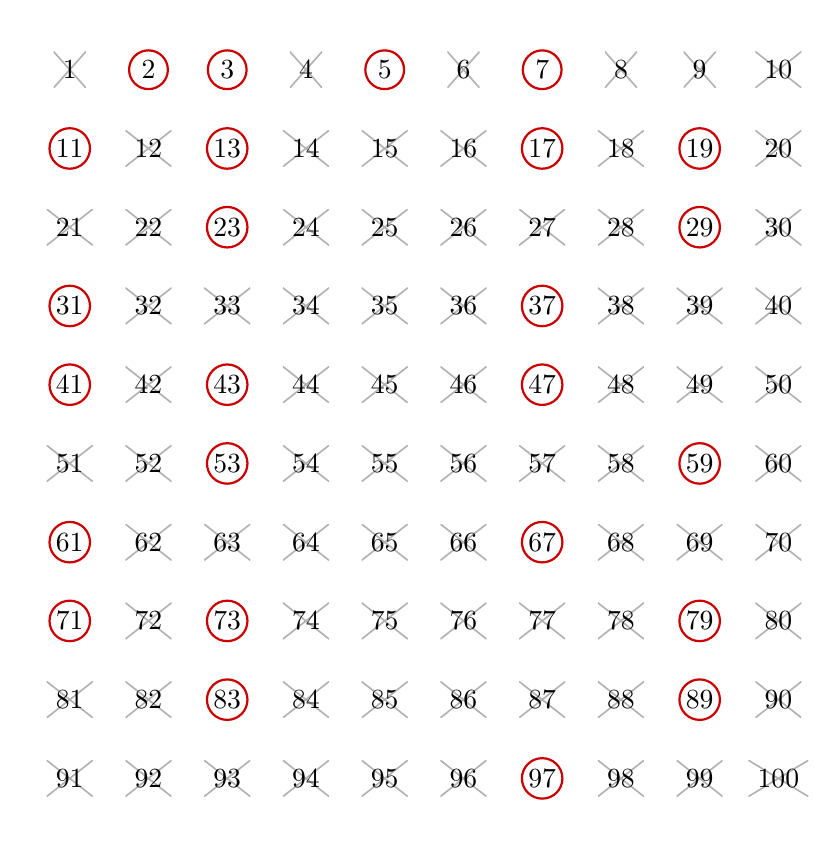
\begin{tikzpicture}[prime/.style={draw=red!80!black, thick, circle, fill=white, inner sep=1pt, minimum size=14pt},crossed/.style={ path picture={ \draw[gray!60, line width=0.6pt] (path picture bounding box.south west) -- (path picture bounding box.north east) (path picture bounding box.south east) -- (path picture bounding box.north west); } } ]
			\foreach \n in {1,...,100} { \pgfmathtruncatemacro{\r}{int((\n-1)/10)} \pgfmathtruncatemacro{\c}{\n - \r*10} \node[crossed] at (\c, 10-\r) {\n}; }
			\foreach \p in {2,3,5,7,11,13,17,19,23,29,31,37,41,43,47,53,59,61,67,71,73,79,83,89,97} { \pgfmathtruncatemacro{\r}{int((\p-1)/10)} \pgfmathtruncatemacro{\c}{\p - \r*10} \filldraw[white] (\c, 10-\r) circle (15pt); \node[prime] at (\c, 10-\r) {\p}; }
		\end{tikzpicture}
	\end{center}
\end{rem}
